\section{DEMONSTRATION}
\label{sec:demonstration}
% a simple tool for multiple choice dataset evaluation and correction
\subsection{Setup} 
We demonstrate our framework with real-world and researchers can apply it to test 
whether a test dataset is comprehensive or not 
and evaluate a model from various aspects online,
%~\footnote{http://adapt.seiee.sjtu.edu.cn:3308/data\_traning/dataset}}, 
We also provide 12 existing popular datasets, These datasets can mainly be classified into two types of tasks. 
The first type are 3 NLI classification tasks (SNLI, QNLI, MNLI), a special case of multiple choice datasets. 
The second type are the multiple choice problems, including ARCT, 
ARCT\_adv\cite{schuster2019towards}, 
RACE~\cite{lai2017race}, and RECLOR~\cite{yu2020reclor}, in which ``hypothesis'' 
is one of the alternatives and ``premise'' contains more than one context roles. 
Ubuntu~\cite{lowe2015ubuntu}, COPA~\cite{roemmele2011choice}, ROCStory, SWAG~\cite{zellers2018swag} and 
CQA~\cite{talmor2019commonsenseqa} also belong to the second type but with only context role 
in ``premise''. We also provide 3 models, fastText, ESIM and BERT, testing on these 12 tasks.

In~\secref{sec:extract}, we choose to use CP as feature metric because from~\figref{fig:d_figure} we find that 
Pearson Correlation Coefficient(PCC) of accuracy deviation score ($\mathcal{D}$)
\begin{equation}
    \mathcal{D} = {Acc} - {Majority}\footnote{Majority is the accuracy with majority voting.}
\end{equation}
between a logistic regression trained with CP and hypothesis-only models (BERT and fastTest) 
is up to 97.17\% for fastText and 97.34\% for BERT which indicates CP is a good feature evaluation score 
for a dataset. 

\begin{figure}[th]
\centering
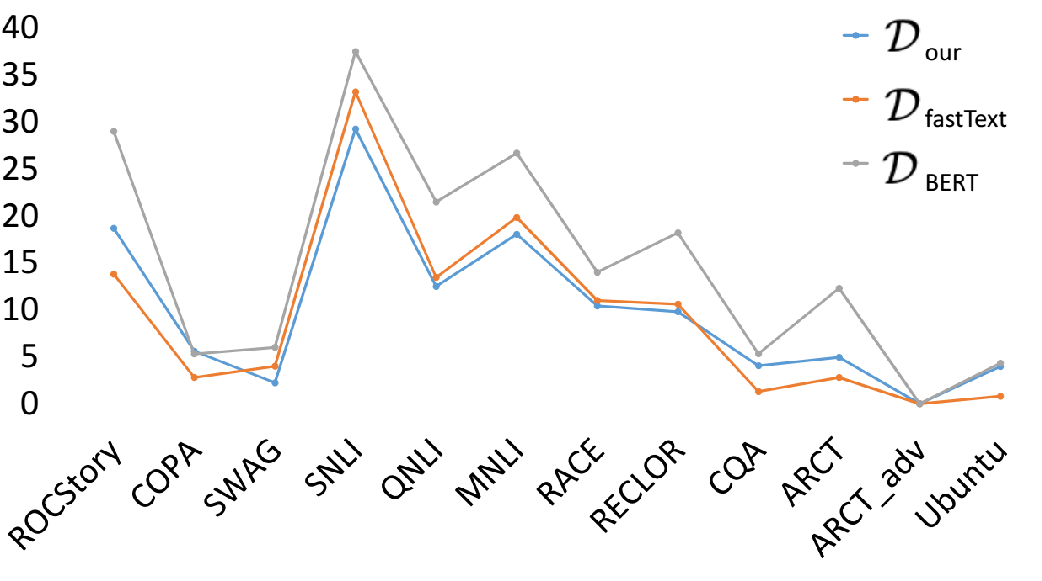
\includegraphics[width=1.0\columnwidth]{picture/d_figure.pdf}
\caption{Deviation scores for three prediction models on all 12 datasets.}
\label{fig:d_figure}
\end{figure}
 In addition, we choose to assign $k$ to 10 which means for Word feature, we only consider 
top 10 works with high feature score. 
The threshold $\sigma$ for decide whether a feature dataset is 
big enough is 5. 

\subsection{Snenarios}
We showcase the following scenarios.
\subsubsection{Dataset Evaluation}

\begin{figure}[th]
\centering
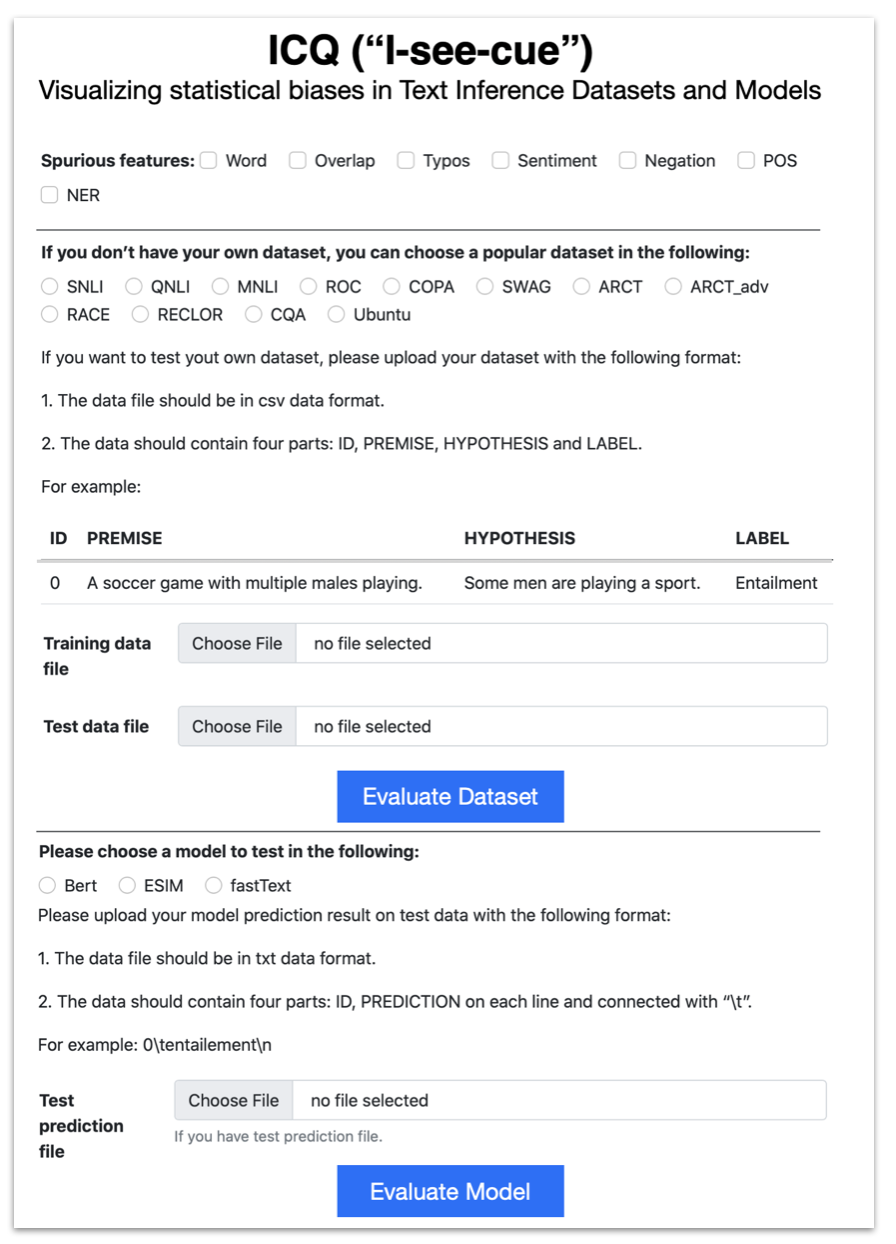
\includegraphics[width=1.0\columnwidth]{picture/dataset.jpg}
\caption{Dataset Evaluation Panel}
\label{fig:dataset}
\end{figure}

We invite the users to experience interactive user interface of our 
framework~\figref{fig:dataset}. Accessing the ``Dataset Evaluation''
panel, users are able to upload their own dataset or select data sources. 
User can also choose the features they really be interested in.
Using  ``Result'' panel, users can view the distribution of training and test dataset 
according to a specific feature. If the KL score is low, it means this feature is a cue. 
For example, in \figref{fig:dataset_result}, we can get to know the distribution of 
each word feature and the similarity between train and test data on this feature with 
KL score.

\begin{figure}[th]
\centering
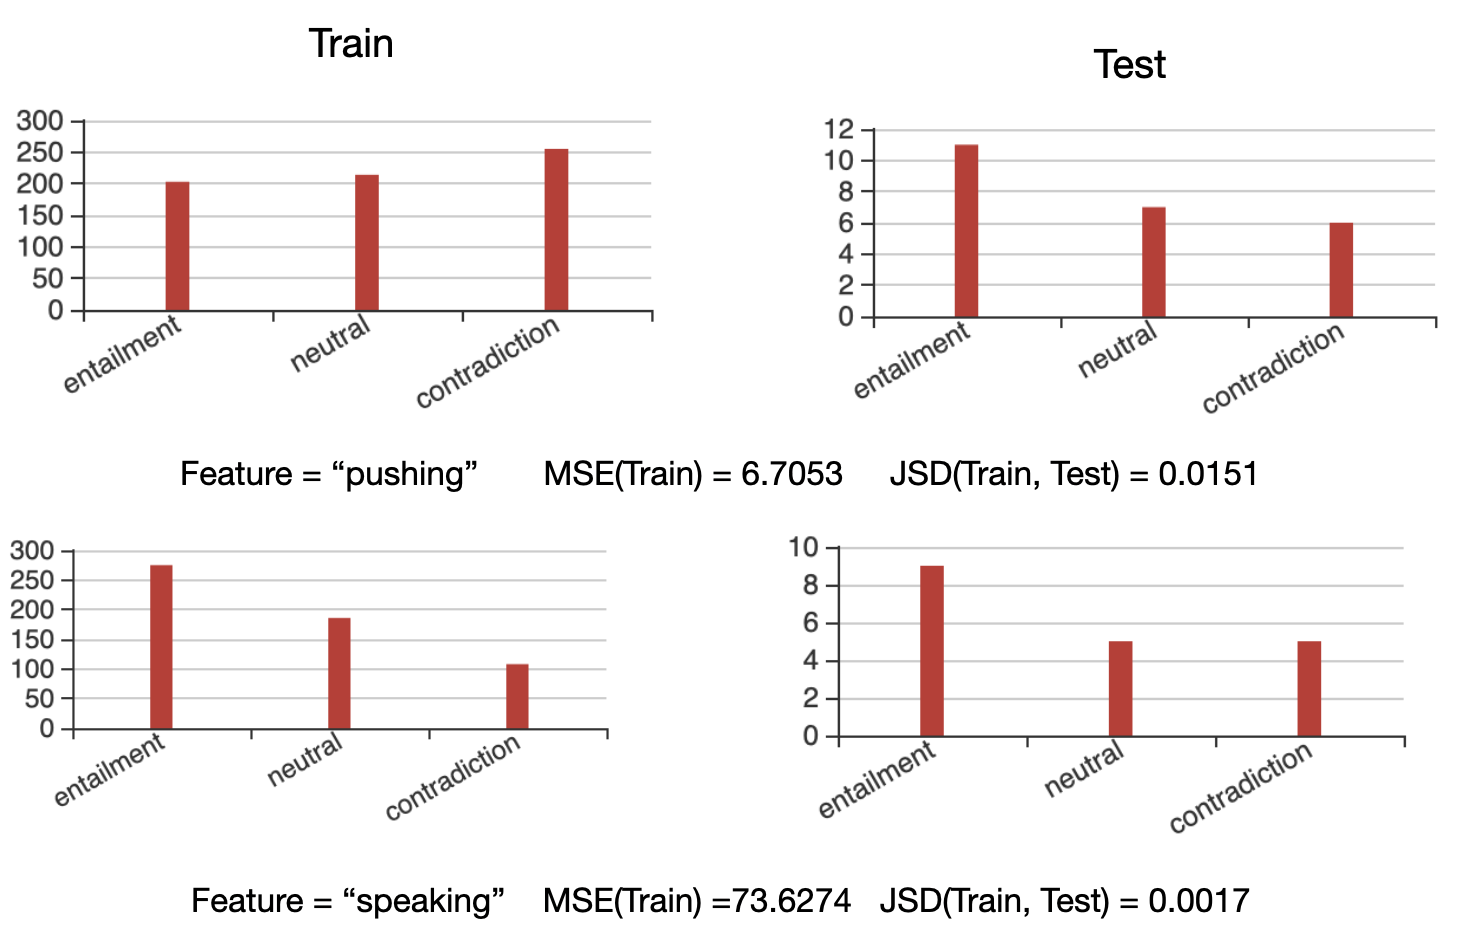
\includegraphics[width=1.0\columnwidth]{picture/dataset_result.jpg}
\caption{Dataset Result Panel}
\label{fig:dataset_result}
\end{figure}

\subsubsection{Model Evaluation}

Over the features which have adequate samples, we also invite the users to 
submit a prediction result file of their model to watch which features is the 
model sensitive to on ``Model Evaluation'' panel. 
In addition, we provide 3 models for our dataset as demo for user 
to test.  Using  ``Model Result'' panel, users can view the distribution of training dataset, 
even-out feature dataset and prediction result of a feature. The KL score is 
calculated between training data distribution and predicting distribution. For example in 
\figref{fig:model_result}, we can find that the Word features are less than before. 
Because we only retain the feature which we have enough test samples with threshold 
$\sigma$.

\begin{figure}[th]
\centering
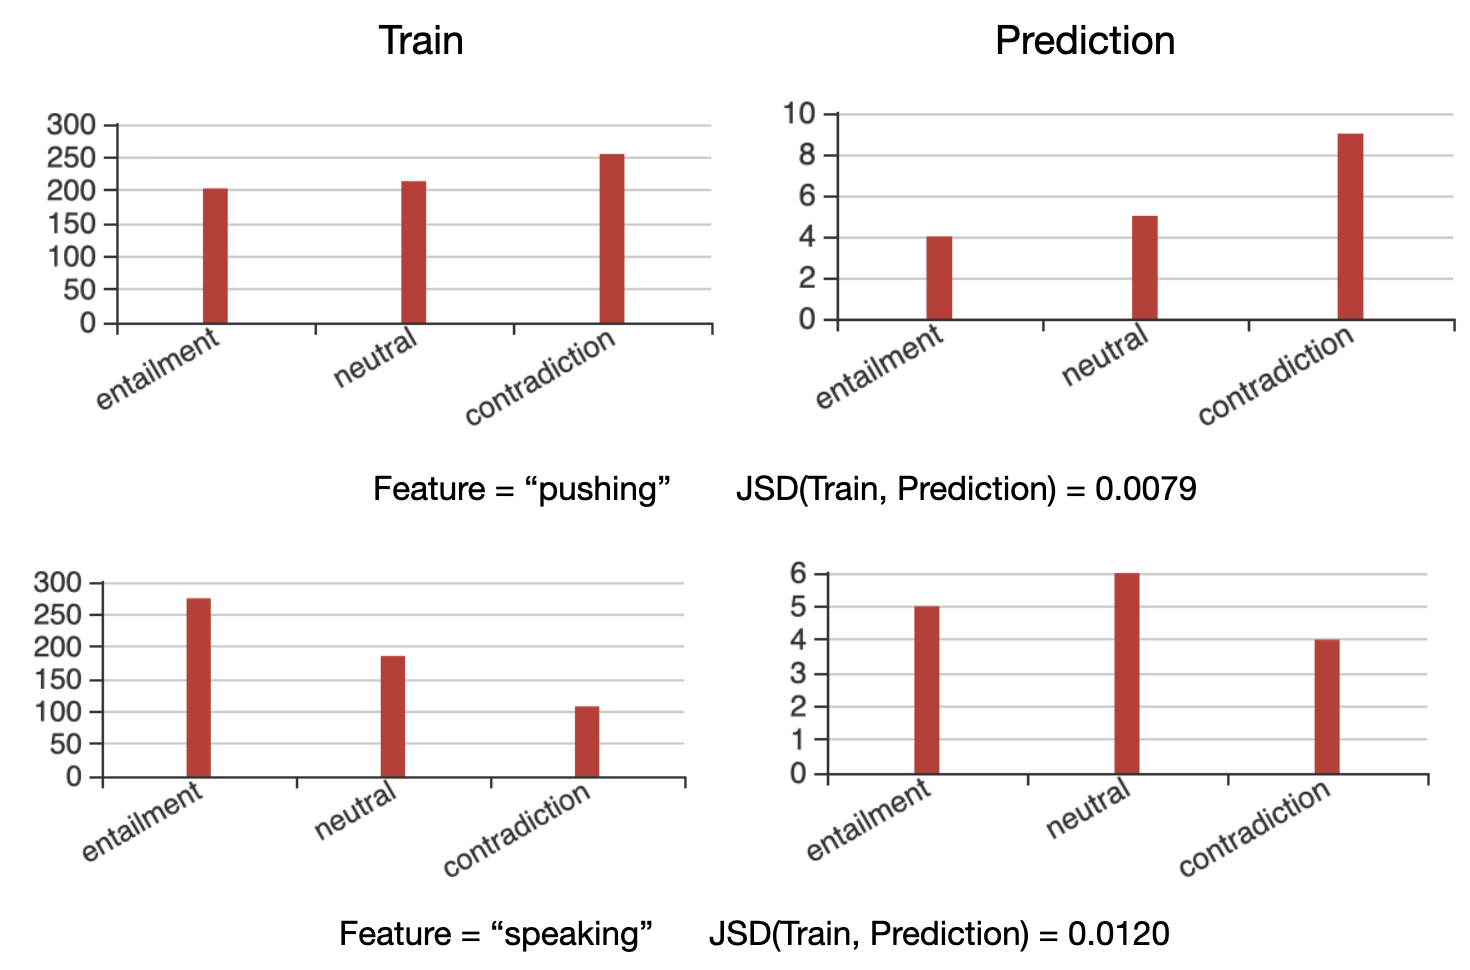
\includegraphics[width=1.0\columnwidth]{picture/model_result.jpg}
\caption{Model Result Panel}
\label{fig:model_result}
\end{figure}
%We proceed to demonstrate the effectiveness of our framework in two aspects:
%First, 
%we use our method to detect cues and measure the amount of information leak
%in 12 datasets from 6 different tasks, as shown in~\tabref{tab:datasets_exp}. 
%Second, we evaluate the true reasoning power of a number of popular NLP
%models on original test sets that are split into 
%easy and hard part. 

%\begin{table*}[th]
%\centering:
%\includegraphics[width=2\columnwidth]{picture/datasets_exp.eps}
%\caption{Data examples and normalized version.}
%\label{tab:datasets_exp}
%\end{table*}
%
% \subsection{Our Results on Different Tasks}
% \label{sec:experiment1}
% 
% We experiment on 12 datasets in \tabref{tab:datasets_exp}. 
% %These datasets are widely used in their 
% %respective fields to provide relevant knowledge and evaluate whether 
%% models have the ability to solve the the problems in a field. %
%%We have give some examples in \figref{fig:datasets_exp}. 
%These datasets can mainly be classified into two types of tasks. 
%The first type are the NLI classification tasks, a special case of multiple choice datasets. 
%The second type are the multiple choice problems, including ARCT, 
%ARCT\_adv\cite{schuster2019towards}, 
%RACE~\cite{lai2017race}, and RECLOR~\cite{yu2020reclor}, in which ``hypothesis'' 
%is one of the alternatives and ``premise'' contains more than one context roles. 
%%\KZ{Don't understand: only has the premise and the hypothesis without the choices.}
%For example, in~\tabref{tab:datasets_exp}, 
%ARCT dataset have \textbf{Reason} and \textbf{Claim} as ``premise'' 
%which requires to select the right warrant between them. 
%%The alternative warrant is the hypothesis and the premise is consist of  reason and claim. 
%%RACE and Reclor includes context and questions which will be seen as ``premise''. 
%%The label for each alternative is 
%%``true'' or ``false'' for whether this hypothesis is the correct one.
%Ubuntu~\cite{lowe2015ubuntu}, COPA~\cite{roemmele2011choice}, ROCStory, SWAG~\cite{zellers2018swag} and 
%CQA~\cite{talmor2019commonsenseqa} also belong to the second type but with only context role 
%in ``premise''.
%
%To show if the word cues really exist in these datasets, 
%we use diverse metrics (in~\secref{sec:approach}) to get cue features. 
%Then we use four simplest ways, the average value classifier (Ave), 
%the maximum value classifier (Max), SGD classifier (SGDC) and 
%logistic regression (LR) (\secref{sec:approach}), 
%to make decision using only the spurious statistical cues. 
%
%
%In order to measure the severity of information leak in data sets, we propose to 
%use the deviation of accuracy from the majority prediction as a measurement which can be expressed as:
%\begin{equation}
%    \mathcal{D} = {Acc} - {Majority}
%\end{equation}
%
%${Majority}$ is the accuracy with majority voting. When the label distribution is balanced, the majority 
%voting is equal to random selection. ${Acc}$ represents the prediction result of 
%a model based on spurious cues only. 
%The difference between our method and the hypothesis-only method (which serves as
%the gold standard here) is that our method uses word-level cues that are interpretable,
%whereas the hypothesis-only method uses more complex cues extracted by advanced models
%which is not interpretable.
%
%
%To track the deviation performance $\mathcal{D}$ of hypothesis-only models,
%we use Pearson Correlation Coefficient(PCC) score to estimate the correlation 
%of deviation results between our methods and hypothesis-only models.  
%We used all the combinations of 8 cue score metrics and 
%4 aggregation algorithms on 12 datasets. We get the 12 deviations of each methods,
%one for each dataset. 
%Meanwhile, we get hypothesis-only deviation results of fasttext and BERT. 
%%Then we calculate all Pearson score between each of our method and hypothesis-only 
%%results. 
%The correlation result is shown in~\tabref{best_method}. 
%We can find that CP cue score with logistic regression model scores 97.17\% 
%with fastText and 97.34\% with BERT which indicates its high correlation 
%with the golden standard hypothesis-only models. 
%Thus we choose CP with logistic regression method to evaluate all datasets in
%the remaining experiments. 
%To further illustrate this trend, we plot $\mathcal{D}$ for 
%our CP+LR method and 2 hypothesis-only models (fastText and BERT) on 12 datasets
%in \figref{fig:d_figure}. 
%wE Can clearly see that the lines are tracking very closely.



